\section{Metodi: ottenere mappe che mostrano il cambiamento}
\label{sec:cambiamento}
A partire dalle mappe di classificazione dell'alveo, si sono ottenute mappe che mostrano come le isole sono, o non sono, cambiate: erosione, crescita, fusione nella \emph{floodplain} o permanenza (nessun cambiamento).
\\
Per ottenere questi dati, ogni mappa è stata confrontata con quella temporalmente precedente.
\\
L'analisi si è focalizzata sulle isole, mentre si è esclusa la piana alluvionale.

\subsection{Limiti}
\label{subsec:camb-limiti}
Alcune mappe hanno una estensione limitata oppure presentano zone con copertura nuvolosa: ciò riduce il numero di confronti possibili per alcuni tratti. 
Dalle 23 immagini satellitari (si veda la \cref{tab:date-orto-sat}) si sono ottenute in media 20~immagini di confronto per tratto (\cref{tab:confronti}).

Inoltre, le immagini \AST{} non sono correttamente georeferenziate e non sono perfettamente sovrapponibili; l'entità di questo scostamento è dell'ordine di qualche cella.
Questo difetto è di grande importanza poiché per poter investigare l'evoluzione temporale delle isole occorre poter osservare nel tempo ogni cella; se questa si sposta da un'immagine alla successiva, il confronto non è più valido.
\\
La soluzione adottata è stata quella di traslare ogni mappa a nord, sud, est o ovest del numero di celle necessario per poterla sovrapporre alla mappa temporalmente precedente.
L'operazione è stata ripetuta per ogni confronto, per ogni tratto, ed è stata verificata visivamente.
Il massimo errore residuo è di 1~cella (\SI{15}{\m}) di scostamento in pochissime zone nei primi tratti (\numrange[range-phrase={ - }]{1}{4}); data la locale topografia montuosa si è preferito ridurre l'errore a tale entità e tenerlo sotto controllo piuttosto di distorcere la mappa con altre misure di georettifica.
L'entità di questo errore è accettabile poiché quasi tutte le isole hanno estensione maggiore di \SI{225}{\m\tothe{2}}.
\\
Le altre immagini sono invece correttamente georeferenziate.

Infine, per poter confrontare immagini a diversa dimensione di cella, come le \AST{} a~\SI{15}{\m} con le \Pl{} a~\SI{0.5}{\m}, è stato necessario ricampionare le immagini con la dimensione minore (ad esempio le \Pl{}) riportandole alla risoluzione di quelle a dimensione maggiore (le \AST{} o le \Se{}).
\\
Nel ricampionamento l'areale delle isole subisce un incremento o una riduzione, così come l'areale della ghiaia e delle altre classi in quanto nelle celle a dimensione maggiore sono presenti numerose celle a dimensione minore, ognuna con un valore diverso (\cref{fig:ricamp-explanation}).
%
\begin{figure}
	\centering
	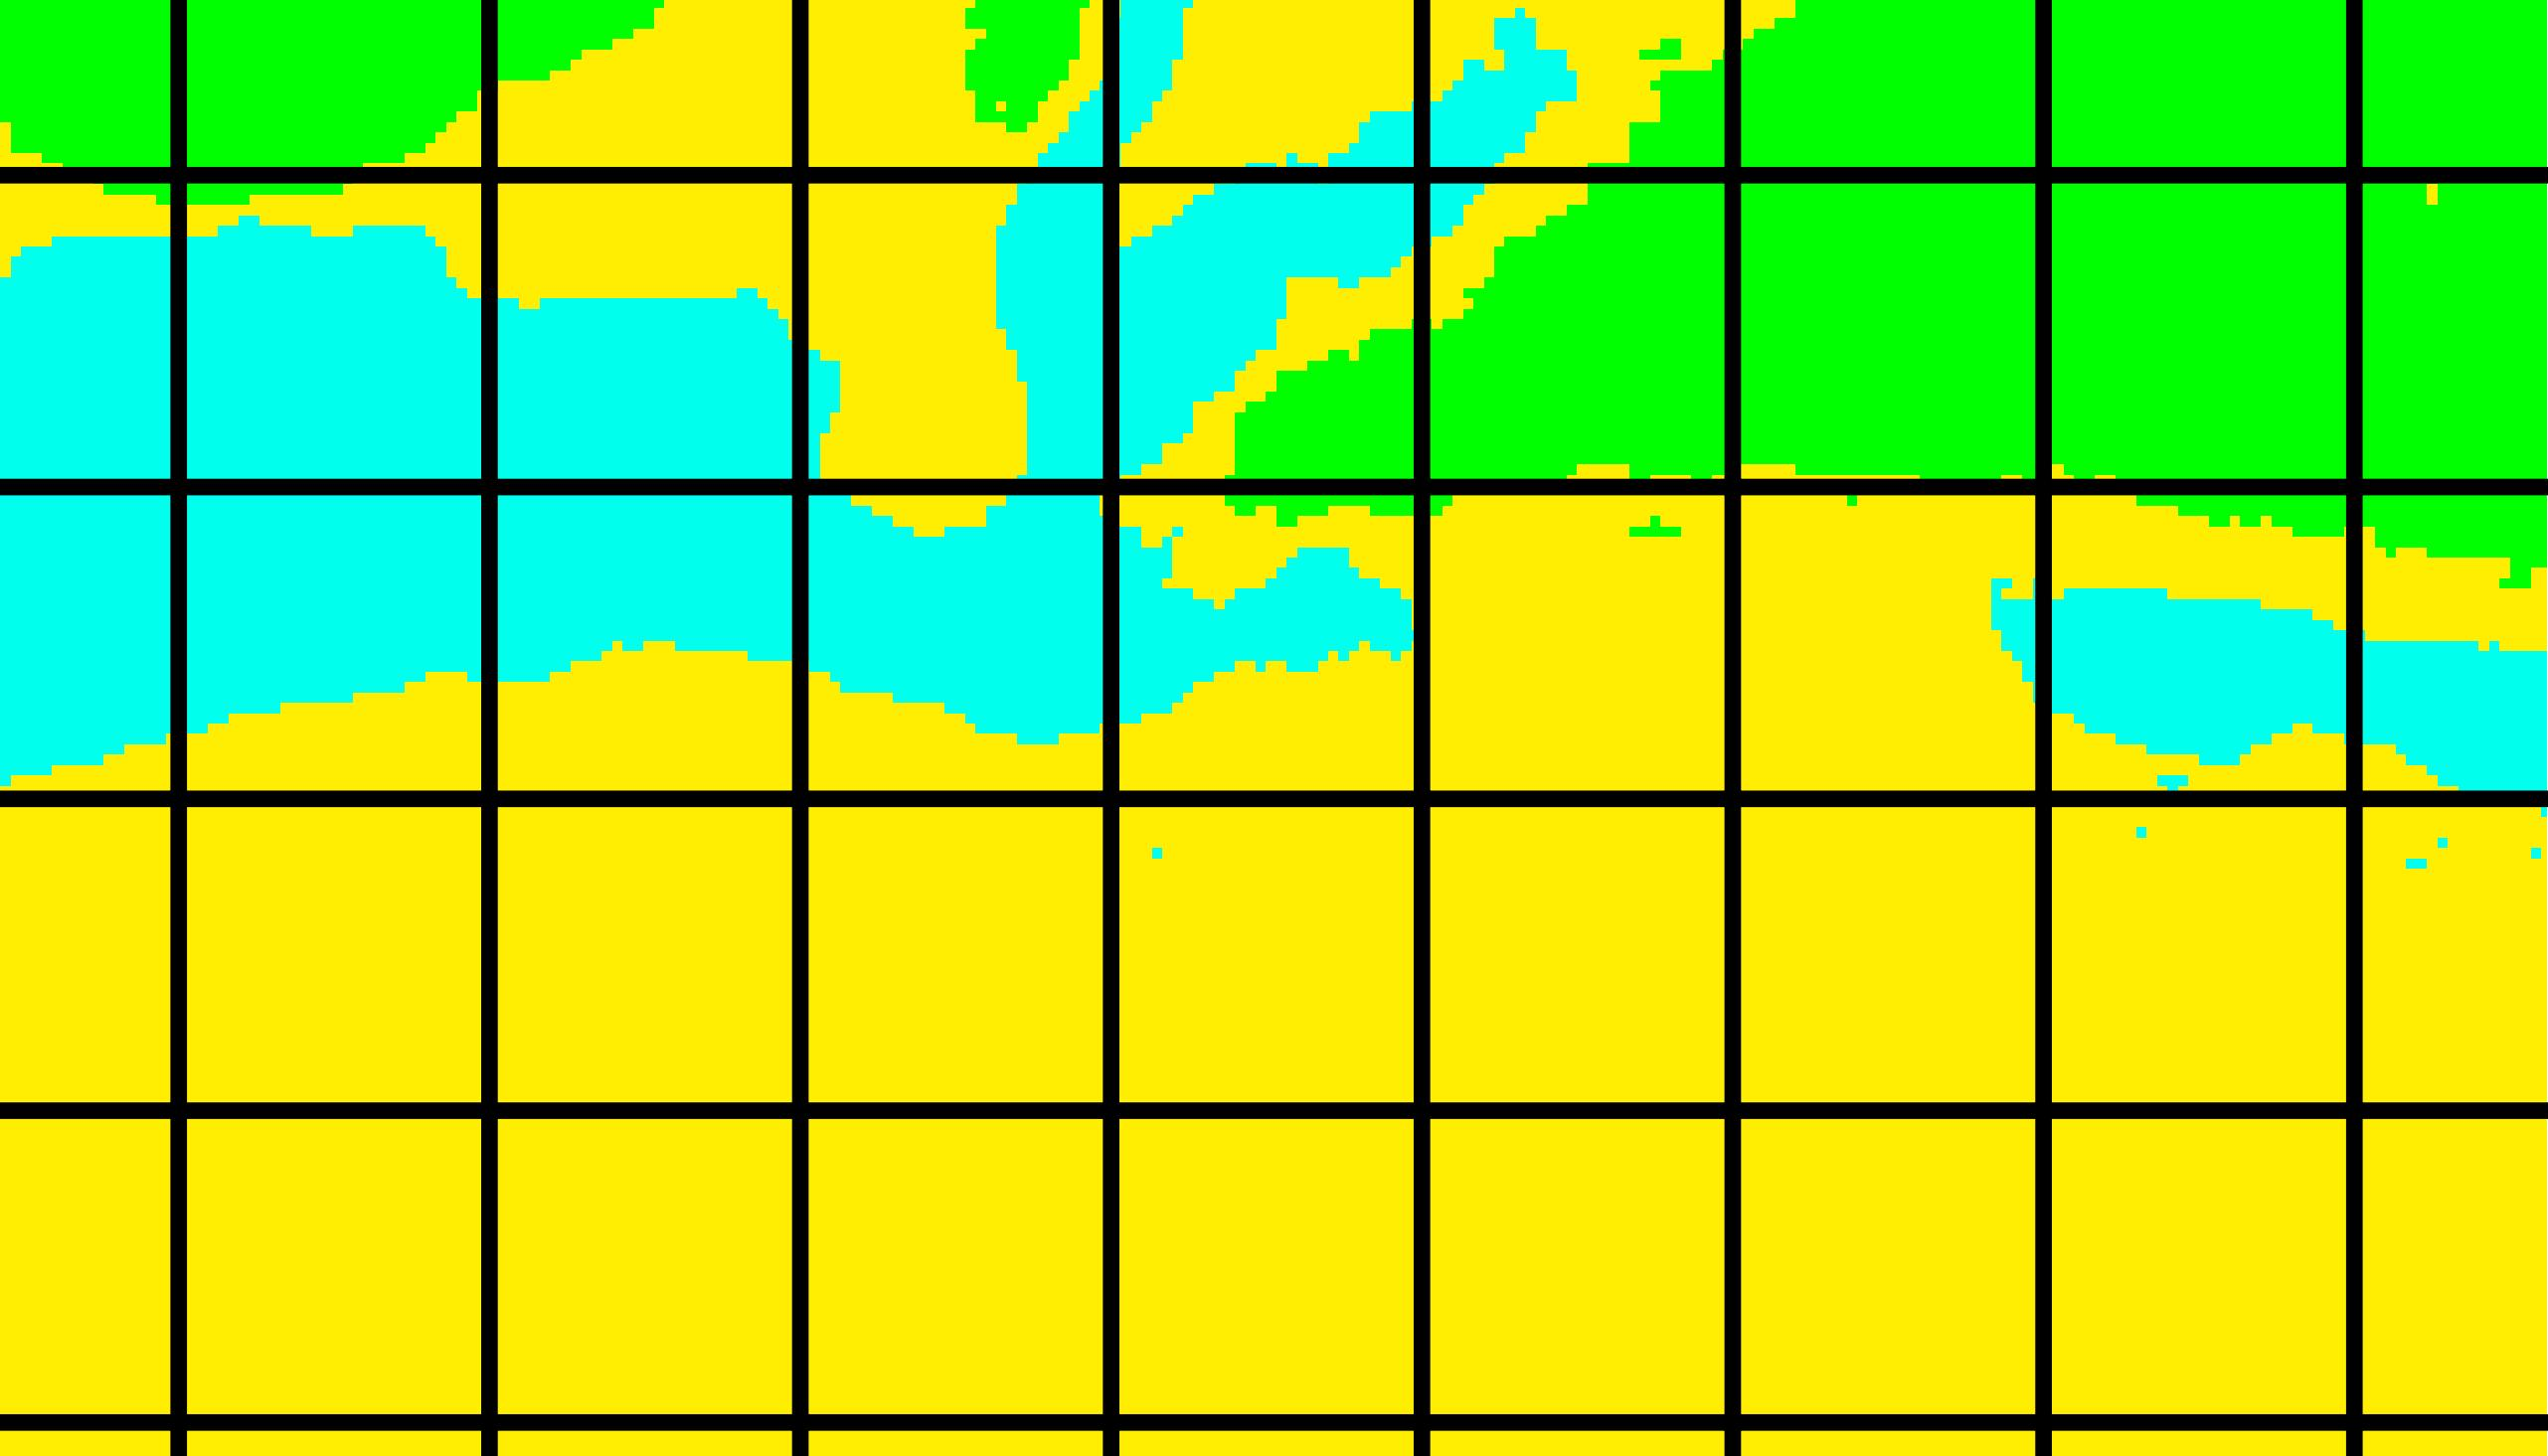
\includegraphics[width=.9\textwidth]{files/ricamp_griglia.jpeg}
	\caption[celle a risoluzione diversa]{immagine \Pl{} 2015-08-13 a~\SI{0.5}{\m} sullo sfondo con la griglia a~\SI{15}{\m} in primo piano; si vede come diverse celle più piccole siano contenute in una singola cella maggiore.}
	\label{fig:ricamp-explanation}
\end{figure}
%
Nel ricampionamento si sceglie quale valore assegnare alla nuova cella più grande in base ai valori delle celle minori; nel presente lavoro si è scelto di assegnare un percentile.
La scelta del percentile è stata effettuata confrontando la radice quadrata della somma dei quadrati residui (RSQR):
%
\begin{equation}
	\label{eq:rad-som-quad-res}
	RSQR = \left\lbrace \sum_{n=1}^{cl} \left[\left( \frac{area_{\mathrm{orig,n}}}{area_{\mathrm{orig,tot}}} - \frac{area_{\mathrm{perc,n}}}{area_{\mathrm{perc,tot}}} \right)^2 \right] \right\rbrace ^ \frac{1}{2}	
\end{equation}
%
dove 
\begin{itemize}
	\item $cl$ è il numero di classi (\cref{tab:class_tratti});
	\item $n$ indica la $n$-esima classe;
	\item $area_{\mathrm{orig,n}}$ e $area_{\mathrm{perc,n}}$ sono l'area della $n$-esima classe rispettivamente nella mappa originale e in quella ricampionata al $perc$-esimo percentile;
	\item $area_{\mathrm{orig,tot}}$ e $area_{\mathrm{perc,tot}}$ sono l'area totale rispettivamente nella mappa originale e in quella ricampionata al $perc$-esimo percentile. 
\end{itemize} 
%
Si è scelto di normalizzare l'area di ogni classe usando come fattore di normalizzazione l'area totale per poter lavorare con percentuali.
\\
Nei ricampionamenti da \SI{0.5}{\m} il $50_\mathrm{mo}$ percentile (mediana) è quello che mostra il minor RSQR ($<\SI{3}{\percent}$). Un esempio del risultato ottenuto è mostrato in \cref{fig:ricampionamento}.
%
\begin{figure}
	\centering
	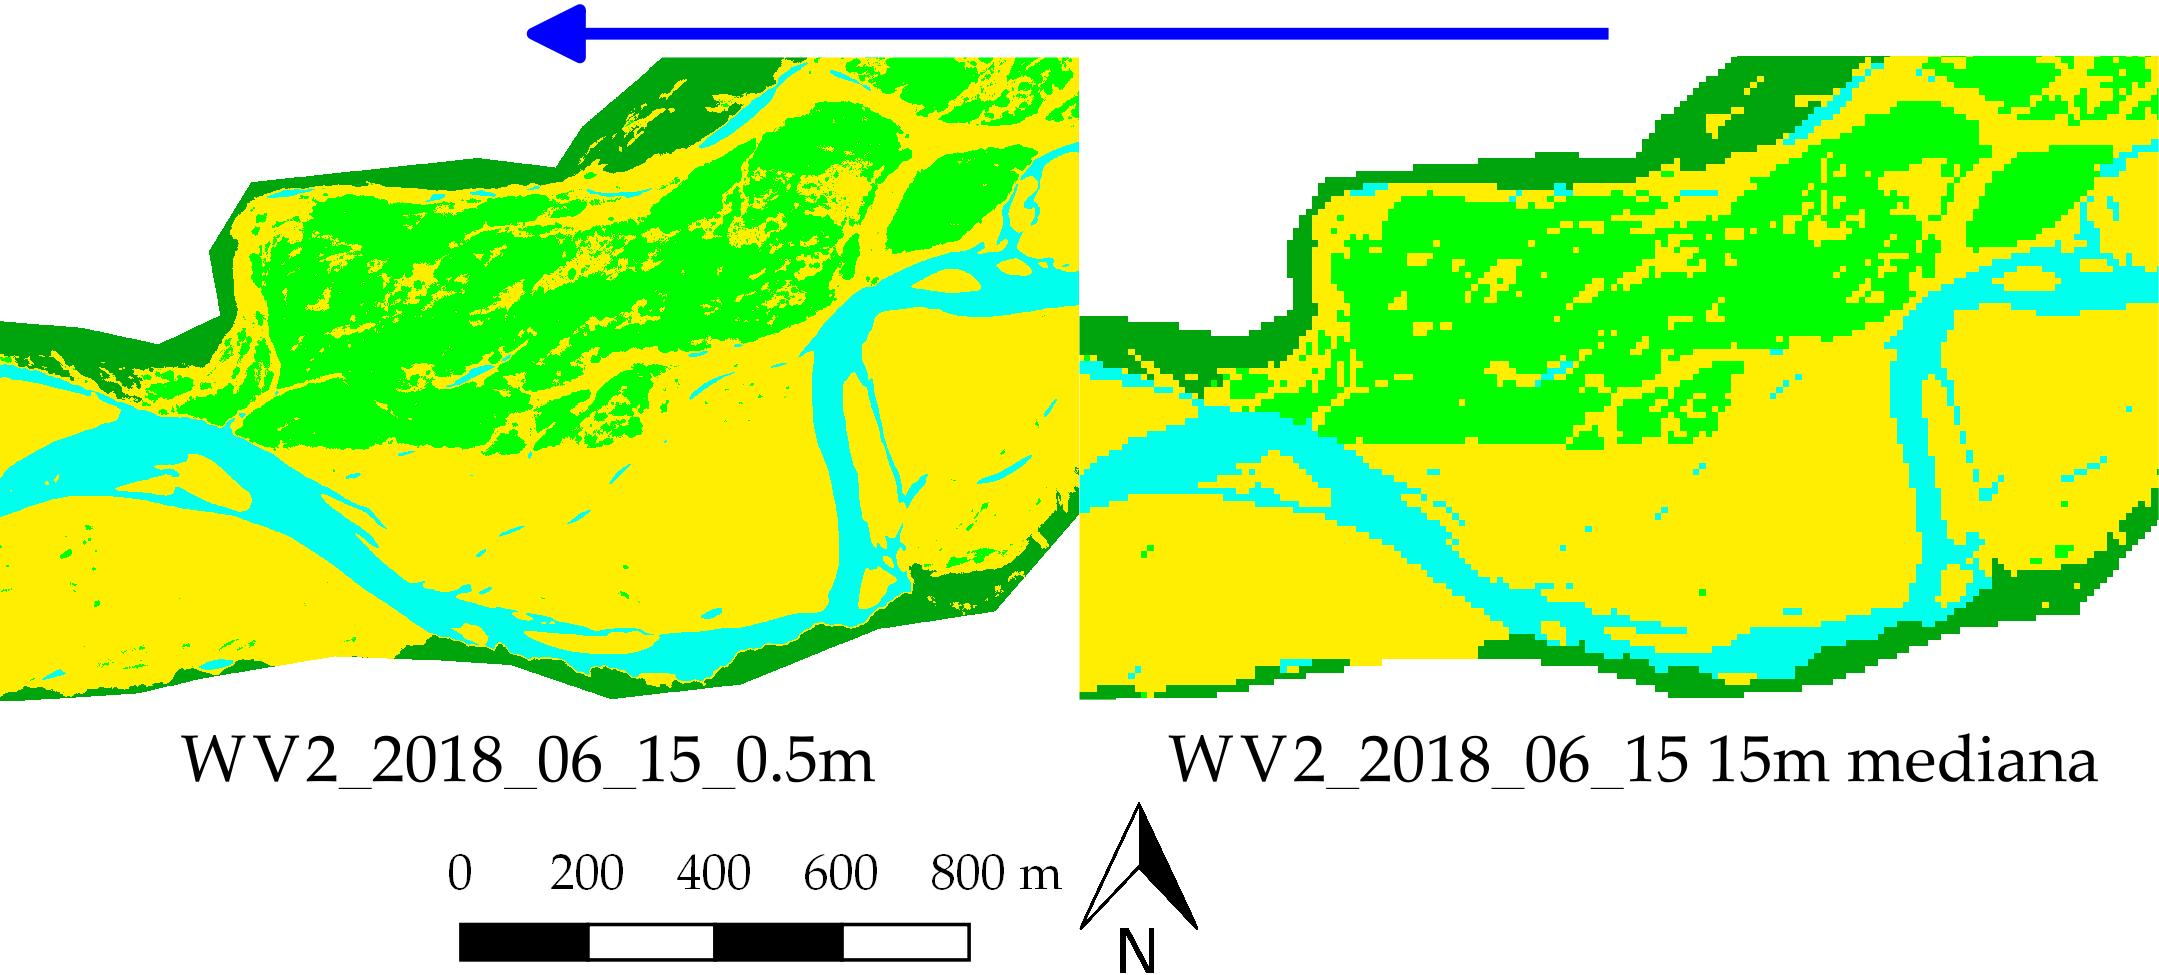
\includegraphics[width=\textwidth]{files/ricamp_class_is_fl.jpeg}
	\caption[confronto originale - ricampionamento]{a sinistra l'immagine \WV{} originale, poco a valle dell'isola di Cornino; a destra la stessa immagine ricampionata distribuendo i valori con la mediana.}
	\label{fig:ricampionamento}
\end{figure} 
%


\subsection{Confronti validi}
Dalle 23 immagini satellitari è stato possibile ottenere il numero di confronti mostrati in \cref{tab:confronti}. 
I confronti effettuati hanno la massima risoluzione temporale possibile, cioè per ogni tratto si sono confrontate le immagini valide temporalmente più vicine, in modo da poter osservare gli effetti cumulati del minor numero possibile di eventi di piena.
%
\begin{table}
	\centering
	\begin{tabular}{
		S[table-format=2.0] 
		S[table-format=2.0]
		c 
		c}
		\toprule
		\textbf{Tratto}	&	\textbf{Confronti}	&	\textbf{Primo}		&	\textbf{Ultimo}	\\
						&	\textbf{validi}		&	\textbf{confronto}	&	\textbf{confronto}	\\
		\midrule
		1	&	17	&	2000-09-17/2002-05-18	&	2017-09-13/2018-09-16	\\
		2	&	18	&	2000-09-17/2002-05-18	&	2017-09-13/2018-09-16	\\
		3	&	19	&	2000-09-17/2001-06-07	&	2017-09-13/2018-09-16	\\
		4	&	19	&	2000-09-17/2001-06-07	&	2017-09-13/2018-09-16	\\
		5	&	19	&	2000-09-17/2001-06-07	&	2017-09-13/2018-09-16	\\
		6	&	23	&	2000-09-17/2001-06-07	&	2018-06-15/2018-09-16	\\
		7	&	23	&	2000-09-17/2001-06-07	&	2018-06-15/2018-09-16	\\
		8	&	23	&	2000-09-17/2001-06-07	&	2018-06-15/2018-09-16	\\
		9	&	22	&	2000-09-17/2002-05-18	&	2018-06-15/2018-09-16	\\
		10	&	22	&	2000-09-17/2002-05-18	&	2018-06-15/2018-09-16	\\
		11	&	21	&	2000-09-17/2002-05-18	&	2018-06-15/2018-09-16	\\
		12	&	21	&	2000-09-17/2002-05-18	&	2018-06-15/2018-09-16	\\
		13	&	22	&	2000-09-17/2002-05-18	&	2018-06-15/2018-09-16	\\
		14	&	23	&	2000-09-17/2002-05-18	&	2018-06-15/2018-09-16	\\
		15	&	19	&	2000-09-17/2002-06-12	&	2017-09-13/2018-09-16	\\
		16	&	19	&	2000-09-17/2002-06-12	&	2017-09-13/2018-09-16	\\
		17	&	19	&	2000-09-17/2002-06-12	&	2017-09-13/2018-09-16	\\
		18	&	19	&	2000-09-17/2002-06-12	&	2017-09-13/2018-09-16	\\
		19	&	19	&	2000-09-17/2002-06-12	&	2017-09-13/2018-09-16	\\
		20	&	19	&	2000-09-17/2002-06-12	&	2017-09-13/2018-09-16	\\
		21	&	19	&	2000-09-17/2001-06-07	&	2017-09-13/2018-09-16	\\
		22	&	19	&	2001-06-07/2002-06-12	&	2017-09-13/2018-09-16	\\
		23	&	19	&	2001-06-07/2002-06-12	&	2017-09-13/2018-09-16	\\
		\bottomrule
	\end{tabular}
	\caption[confronti effettuati]{confronti effettuati con le 23 immagini satellitari a disposizione per ottenere dati sul cambiamento delle isole.}
	\label{tab:confronti}
\end{table}
%

\subsection{Classi di cambiamento}
In ogni confronto ci si è concentrati su ciò che è successo alle isole, definendo quindi le seguenti 4~classi (si veda anche la \cref{tab:class_tratti}):
%
\begin{itemize}
	\item erosione (da isola ad alveo attivo);
	\item crescita (da alveo attivo ad isola);
	\item fusione nella \emph{floodplain} (da isola a \emph{floodplain});
	\item distaccamento dalla \emph{floodplain} (da \emph{floodplain} a isola);
	\item nessun cambiamento (da isola a isola).
\end{itemize}
%
Un esempio di questa classificazione è riportato nella \cref{fig:confr-class-is-fl}.
%
\begin{figure}
	\centering
	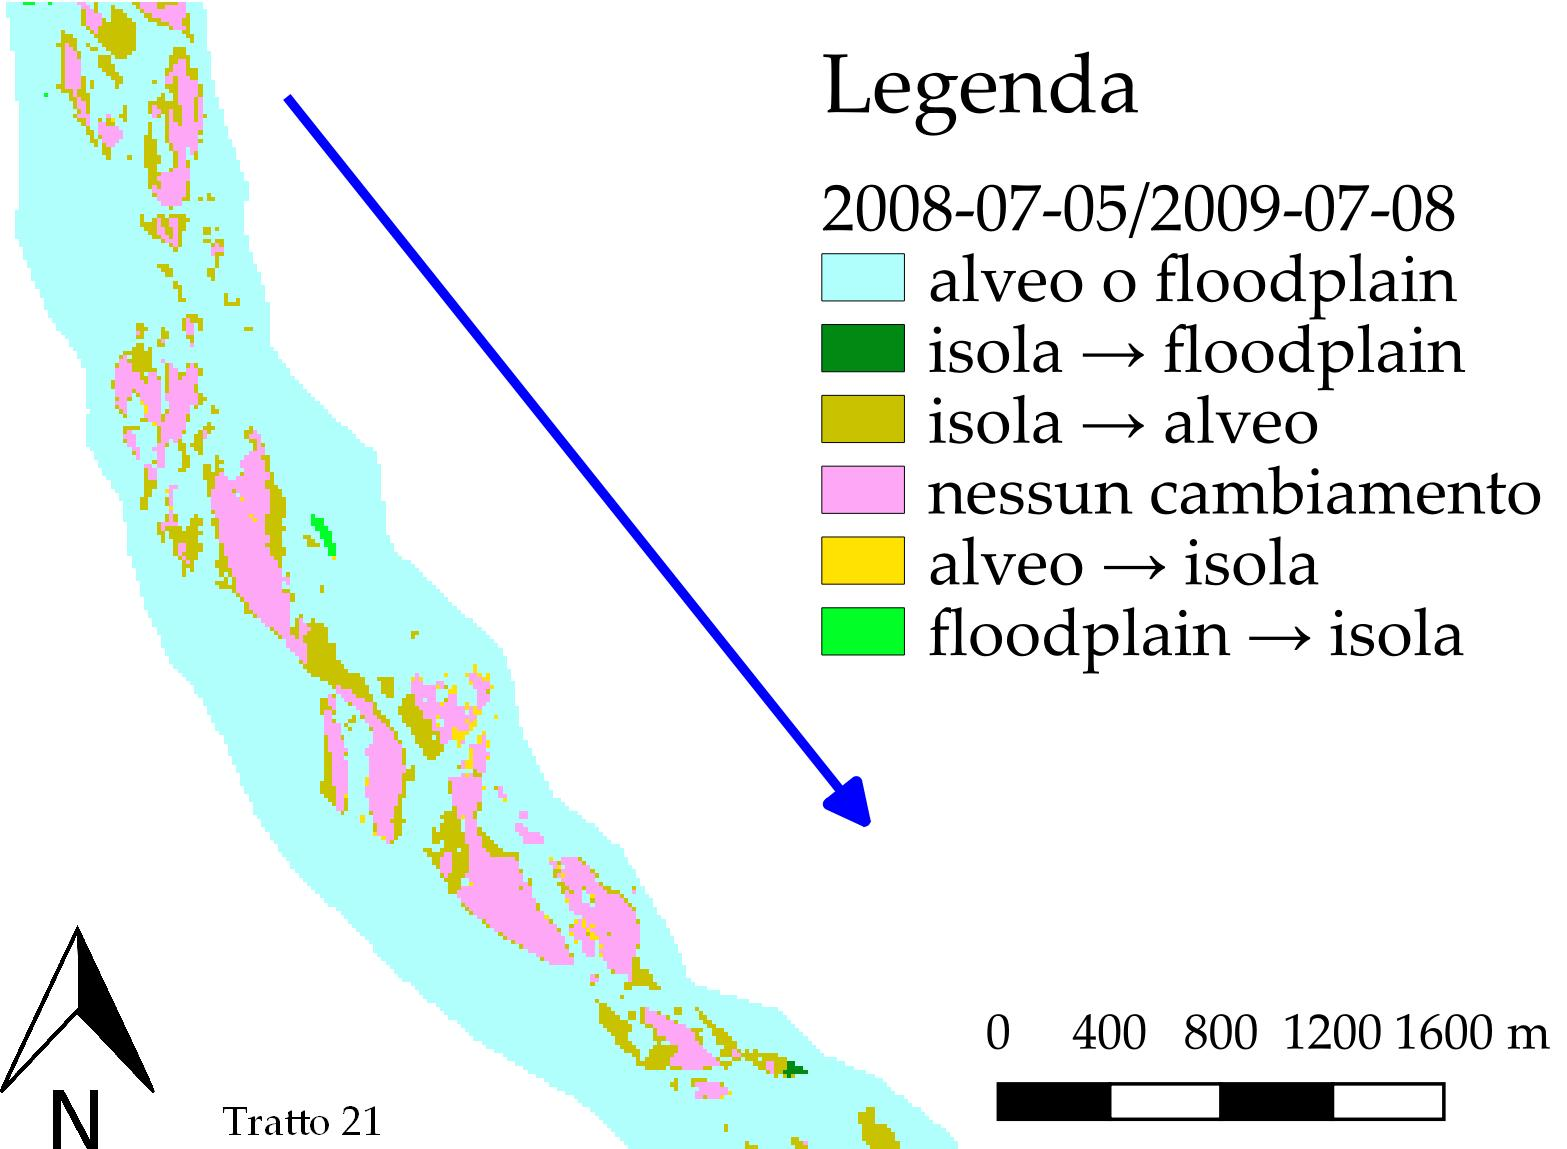
\includegraphics[width=.8\textwidth]{files/confr_class_is_fl.jpeg}
	\caption[esempio di mappa di cambiamento]{esempio di mappa di cambiamento ottenuta con il confronto tra le immagini \AST{} 2008-07-05 e 2009-07-08. Si possono osservare tutti i cambiamenti possibili; la prima classe, colorata in azzurro, visualizza l'area dell'intera maschera computazionale, e comprende perciò sia l'alveo che la \emph{floodplain}. Il tratto mostrato è posto qualche \si{\kilo\m} a monte del ponte di Madrisio.}
	\label{fig:confr-class-is-fl}
\end{figure}
%

